
\begin{figure}
    \centering
    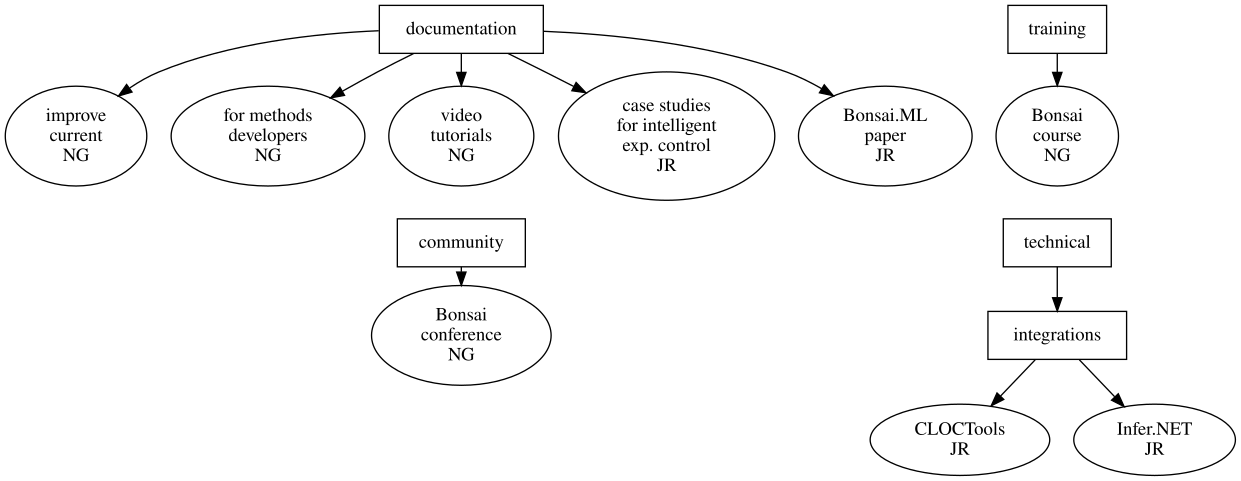
\includegraphics[width=6in]{activitiesGraphs/activities_larger.png}
    \caption{Proposed activities. See text for details.}
\end{figure}

\subsection*{Approach}

\subsubsection*{Documentation}

\paragraph{Summary:} Expand Bonsai.ML documentation.

\paragraph{Previous work:} Bonsai.ML already contains substantial
\href{https://bonsai-rx.org/machinelearning/index.html}{documentation} for all
distributed packages. This documentation includes Bonsai working examples that
users can copy and paste them in their Bonsai local runtime and execute them.

\paragraph{Subtasks (responsible team member):}\mbox{}\\
\begin{itemize}

    \item\textbf{provide more examples (NG)} on the application of the already
        integrated ML methods to new types of behavioural and neural data.
        %
        These examples will be similar to the
        \href{https://bonsai-rx.org/machinelearning/examples/README.html}{existing
        ones}, but they will be more detailed.

    \item\textbf{include video tutorials (NG)} on the use of the Bonsai.ML
        package.

    \item\textbf{add documentation for methods developers (NG)} as the current one is
        targeted to Bonsai.ML users.

    \item\textbf{create case studies (JR)} for intelligent experimental control
        in Bonsai, similar to the
        \href{https://mark-kramer.github.io/Case-Studies-Python/intro.html}{case
        studies for neural data analysis in Python}, or those for
        \href{https://mbmlbook.com/index.html}{model based machine learning},
        by our Microsoft collaborators.

    \item\textbf{publish a first Bonsai.ML paper (NG)} describing its functionality, as
        companion papers substantially increases the adoption of software
        packages \citep{lopesEtAl15,guilbeaultEtAl21}.

\end{itemize}

\noindent\rule{\textwidth}{1pt}
\subsubsection*{Training}

\paragraph{Summary:} Organise Bonsai course, with Bonsai.ML module.

\paragraph{Previous work:} Since 2017, NeuroGEARS Ltd (the non-profit
organisation that is the main contributor to the development of Bonsai) has
organised at least two Bonsai course per year at different universities, and
\href{https://bonsai-rx.org/learn/}{some of them} can be viewed
online.

\paragraph{Outputs:} course delivery, online course material.

\paragraph{Responsible team members:} GL, NG, JR.

\noindent\rule{\textwidth}{1pt}
\subsubsection*{Collaborations}

\paragraph{Collaboration 1: forecasting animal behaviour for zero-lag stimulus
presentation in augmented-reality experiments.} Prof.~Aman Saleem,
\href{https://www.saleemlab.com/}{Saleem Lab}, Institute of Behavioural
Neuroscience, University College London, UK.


\begin{description}

    \item[Background:] In augmented reality experiments, particularly in
        neuroscience, precise stimulus timing is critical, yet unavoidable
        system delays mean that visual stimuli often appear slightly later than
        intended. This latency is especially problematic when linking neural
        activity to sensory input or behaviour. To address this, we will use
        algorithms that forecast animal position and head orientation, allowing
        stimuli to be pre-rendered and displayed in synchrony with the
        subject's actual position and head orientation.

    \item[Previous work:] In the 2024 Bonsai conference we began conversations
        with Prof.~Saleem about using predictive algorithms, like state-space
        models, to improve augmented reality experiments in animals. We
        implemented in Python a
        \href{https://github.com/joacorapela/collaborationAman/blob/master/reports/ekfForKinematicsAndHeadOrientation/ekfForKinematicsAndHeadOrientation.pdf}{
            nonlinear state-space model, and the extended Kalman filter
            algorithm} to estimate the model parameters, in order to forecast,
        using video recordings, position and head orientation of mice exploring
        a circular arena surrounded by a 360 degree visual display screen. We identified
        experimental and methodological improvements for the next iteration of
        the collaboration.

    \item[Future work:] We will to further test the accuracy of the previous
        model and estimation algorithm and, if needed, explore alternatives. For
        this we will use artificially generated data with ground truth. The
        Saleem laboratory will improve experimental issues. Then we
        will evaluate the performance of the Bonsai.ML forecaster in animal
        behavioural data.

    \item[Outcomes:] We will document the activities of the collaboration, create a new
        Bonsai.ML forecasting package, and publish the outcomes of the
        collaboration in a scientific journal.

    \item[Responsible team member:] JR.

\end{description}

\paragraph{Collaboration 2: estimating latent variables for high-channel-count
Neuropixels recordings, in real time, while recordings are being performed.}
Dr.~Josh Siegle, head of the electrophysiology group, Allen Institute for
Neural Dynamics, US.

\begin{description}

    \item[Background:] Visualisation is central to scientific inquiry,
        especially in neuroscience. Yet, modern high-density recordings from
        hundreds or thousands of electrodes pose major challenges for clear,
        real-time visualisation. At the Gatsby Unit, we pioneered single-trial
        dimensionality reduction with latent-variable models \citep{yuEtAl09},
        and extended these approaches in later work, e.g.
        \citep{dunckerAndSahani18}, supported by open-source software
        (\href{https://github.com/joacorapela/svGPFA}{svGPFA}). However, all
        current latent-variable methods operate offline, after data collection.
        In this project we will integrate a state-space model into Bonsai.ML to
        estimate and visualise latent variables online, during
        high-channel-count recordings.

    \item[Previous work:] We have developed a
        \href{https://joacorapela.github.io/ssm/auto_examples/neuralLatents/plot_MC_MAZE_SMALL.html#sphx-glr-auto-examples-neurallatents-plot-mc-maze-small-py}{linear-dynamical-systems
        model and estimation methods to infer latent variables in real time
        from high-channel-count electrophysiological recording}, and we are now
        integrating it into Bonsai.ML.


    \item[Future work:] Evaluate the real-time performance of the Bonsai.ML
        latents estimation method with previously recorded data replayed in
        real time, and later with live neural recordings. Publish a Bonsai.ML
        neural latents package, and a related paper reporting scientific
        findings with the new package.

    \item[Responsible team member:] NG.

\end{description}

\noindent\rule{\textwidth}{1pt}
\subsubsection*{Integrations}

\subsubsection*{Probabilistic programming: Infer.NET}

\paragraph{Background:} Most of the probabilistic models currently integrated
into Bonsai are implemented in Python. These serve as excellent demonstrations
of how Python applications can connect to the Bonsai ecosystem, and they are
central to our aim of attracting Python developers to contribute to Bonsai.ML.

However, Python implementations are substantially slower than equivalent C\#
code. For demanding real-time applications, C\# implementations are preferable,
especially when expressed in a probabilistic programming language (PPL).

The existing Python and C\# implementations of probabilistic models (e.g.,
linear dynamical systems, hidden Markov models, Bayesian linear regression —
see
\href{https://bonsai-rx.org/machinelearning/examples/README.html}{examples})
are relatively complex and heterogeneous, making them harder to maintain. In
contrast, implementations in a C\# PPL would be faster, simpler, and more
homogeneous, reducing errors and improving maintainability.

Fortunately, C\# has an excellent PPL:
\href{https://dotnet.github.io/infer/}{Infer.NET}, developed at Microsoft
Research Cambridge since 2004, used in
\href{https://dotnet.github.io/infer/papers.html}{hundreds of papers}, and
\href{https://www.microsoft.com/en-us/research/blog/the-microsoft-infer-net-machine-learning-framework-goes-open-source/}{open-sourced
in 2018}.  Infer.NET uses deterministic approximate inference, enabling fast
and scalable solutions. For
\href{https://www.microsoft.com/en-us/research/blog/the-microsoft-infer-net-machine-learning-framework-goes-open-source/}{example},
it has powered systems that extract knowledge from billions of web pages
(petabyte-scale data) — the kind of scalability critical for real-time
inference in Bonsai.

Message passing is a natural connection point between Bonsai and Infer.NET.
Infer.NET uses message passing for approximate inference, while Bonsai relies
on message passing for reactive computations. Exposing Infer.NET’s message
passing algorithms as Bonsai nodes will allow users to seamlessly combine
efficient inference with reactive experimental control.

We will re-implement in Infer.NET all the probabilistic models previously
integrated into Bonsai using Python or C\#. This integration will accelerate
inference, simplify and standardise inference programs, and empower Bonsai
users to create new probabilistic models and inference algorithms with just a
few lines of code. By making powerful yet easy-to-use inference methods
accessible to experimental neuroscientists, this project has the potential to
profoundly advance scientific discovery.

\paragraph{Previous work:} Our Microsoft collaborator, Dr.~Tom Minka, invented
a seminal algorithm for inference in graphical models, the Expectation
Propagation algorithm~\citep{minka01}, and is the lead developer of Infer.NET.
Please refer to his letter of support.

\paragraph{Responsible team member:} JR.

\paragraph{Outputs:}\mbox{}\\

\begin{itemize}

    \item Bonsai nodes implementing Infer.NET inference methods
    \item online Bayesian linear regression implemented in Bonsai.ML--Infer.NET
    \item linear dynamical systems implemented in Bonsai.ML--Infer.NET
    \item hidden Markov model implemented in Bonsai.ML--Infer.NET
    \item point-process decoder implemented in Bonsai.ML--Infer.NET
    \item documentation, tutorials and use cases on how to work with
probabilistic programming models in Bonsai--Infer.NET \end{itemize}

\subsubsection*{Closed-loop optogenetic control tools: CLOCTools}

\paragraph{Background:} Closed-loop neural control represents a transformative
advance in neuroscience:  rather than delivering stimulation at fixed,
open-loop schedules, it enables precisely timed interventions based on ongoing
brain and behavioural activity. This paradigm allows researchers to move beyond
observing correlations to  directly testing causal mechanisms of neural
dynamics, plasticity, and behaviour. Critically, closed-loop stimulation has
already proved transformative in the  clinic, for example in deep brain
stimulation for Parkinson’s disease and  epilepsy, while its extension to other
disorders (e.g. depression, obsessive  compulsive disorder) remains an active
area of research. Despite this promise, widespread adoption has been limited
by the lack of accessible, well-engineered,  and sustainable software
frameworks for real-time experimental control.

Prof.~Garrett Stanley (Georgia Tech, US) is a pioneer in closed-loop
neuroscience, having developed groundbreaking methods that combine real-time
neural control with systems neuroscience. He recently contacted us to explore
integrating their existing \href{https://cloctools.github.io/}{CLOCTools},
originally implemented in RTXI/C++, into Bonsai.ML.  This represents a unique
opportunity: Bonsai already excels at real-time closed-loop control in
behavioural experiments, and extending it to include state-of-the-art
closed-loop neural control will position the platform as the first sustainable,
general-purpose framework for both levels of experimentation.

An important reason for the poor uptake of closed-loop methods in neuroscience
could be that existing implementations are often ad hoc, difficult to install
or  extend, and not integrated with modern pipelines for data analysis or
sharing. By providing Bonsai users with accessible, open-source, and
sustainably engineered tools for closed-loop control, we will directly address
this barrier and enable a new type of experimentation where researchers can
both read and write the neural code in real time. This will accelerate
discovery across both basic and translational neuroscience.

\paragraph{Previous work:} Members of Prof.~Stanley’s lab have already
prototyped some of their closed-loop control methods in Bonsai using our
\href{https://bonsai-rx.org/python-scripting/}{Python scripting interface}.

\paragraph{Responsible team members:} JR

\paragraph{Subtasks:}\mbox{}\\

\begin{itemize}

    \item collaborate with the group of Prof.~Stanley on the implementation in
        C\# the functionality in the repository
        \href{https://github.com/CLOCTools/lds-ctrl-est}{lds-ctr-est}.

    \item deploy a comprehensive battery of test cases to check the correctness
        of the C\#/Bonsai implementation against the C++/RTXI one.

    \item reproduce in C\# all the tutorials and examples in the repository
        lds-ctr-est.

    \item develop addition documentation, tutorials and use cases for
        experimental neuroscientists with no training on feedback control.

\end{itemize}

\noindent\rule{\textwidth}{1pt}
\subsubsection*{Governance}

We will create a Bonsai.ML steering committee that will provide us strategic
oversight on this project and advise us on building a long-term development
roadmap for Bonsai.ML.

Several renowned experimental and computational neuroscientists around the
world are heavily invested in Bonsai, are very interested in adding ML
functionality to their Bonsai workflows and have agreed to join the Bonsai.ML
steering committee. We list them below.

\begin{description}

    \item[Prof.~Thomas Mrsic-Flogel,] director of the SWC, project lead on the
        BBSRC grant that funded the creation of Bonsai.ML, and project lead on
        this proposal. Bonsai is the main software for experimental control at
        the SWC.

    \item[Prof.~Maneesh Sahani,] director of the GCNU, project co-lead on the
        BBSRC grant that funded the creation of Bonsai.ML, and project co-lead
        on this proposal.

    \item[Prof.~Aman Saleem,] director of the Saleem Lab at the Institute for
        Behavioural Neuroscience, University College London. Prof.~Saleem is the
        author of \href{https://bonvision.github.io/}{Bon-Vision}, a software
        package that creates and controls visual environments in close loop,
        built on top of Bonsai.

    \item[Prof.~Josh Siegle,] senior scientist and lead of the
        electrophysiology group at the Allen Institute for Neural Dynamics,
        where Bonsai is the only software for experimental control.

    \item[Prof.~Ken Harris,] co-director of the Cortexlab, University College
        London, and founding director of the International Brain Laboratory,
        that uses Bonsai for reproducible experimental control across 22
        laboratories around the world.

    \item[Prof.~Athena Akrami,] director of the Learning, Inference and Memory
        Lab, at the SWC, that uses Bonsai for experimental control.

    \item[Prof.~Garrett Stanley,] leader of the Laboratory for the Control of
        Neural Systems, Georgia Tech, US. Expert on close-loop control of
        neurophysiological systems. He contacted us to migrate to Bonsai
        a package for real-time cortical state estimation and the CLOCTools
        referred above, both originally written in C++/RTXI.

\end{description}

\noindent\rule{\textwidth}{1pt}
\subsection*{Management}

We will conduct management activities at different frequencies:

\begin{description}

    \item[Twice a year:] we will generate a progress report, which will be
        publicly available, and hold meetings with the steering committee to
        discuss it and receive expert advise. Minutes from these meeting will
        be published openly to maintain transparency.

    \item[Every three months:] we will hold meetings between the project lead, TMF, the
        project co-lead, MS, the senior RSE, JR, the junior RSE, NG, and
        the external project co-lead, GL, to evaluate the project progress.

    \item[Weekly:] as has been our practice since the start of the Bonsai.ML
        project, the junior and senior RSEs will meet with the external project
        co-lead to discuss issues that appeared during the week, review
        activities for the following week, and adjust project directions.

    \item[Daily:] the offices of the senior and junior RSEs are next to each
        other, enabling discussions to manage spontaneous project issues.

\end{description}

Meetings with collaborators will be arranged as needed.
%
At the SWC, GCNU and NG we are experimental and computational neuroscientists
with successful collaborative experience, and we have no doubt that the
proposed collaborations will be of the same kind,
%
specially since we have successfully interacted in the past with most of the
propose collaborators.
%
Please refer to their letters of support.
